\chapter{Results}\label{chap:results}

\todo[inline]{results interpretation}
\todo[inline]{results speed up in percentages}
\section{Problem Data and Result Explanation}
\begin{comment}
Existing computer code (written in C++) already exist for the TA algorithms,
including the path equilibrium method and many others.
A simple shortest path calculation algorithm is currently used by the path equilibrium method,
which runs very poorly given a small network.
\end{comment}
\todo{talk about existing code}

The problem data for solving the TA problems are retrieved from Transportation Network Test Problems \citep{ProblemData}.

Through out the report, Table~\ref{table:problemdata} is used to show the run time and number of iterations for solving one particular network.
In the table, the ``OD pairs'' column gives the number of pairs of origin and destination in the network.
The ``zone'' column gives the number of traffic zones,
in some cases, the nodes in the network also include the traffic zones.
The ``Run time (seconds)'' gives is measured from executing the whole 
path equilibration algorithm from start to finish.
The ``Iterations'' column gives how many times the whole network
gets solved to settle the traffic flows to equilibrium.
\todo[inline]{need to explain what an iteration where it is introduced} 
\begin{table}[H]
    \centering
    \begin{tabular}{lrrrr} \toprule
        Network & Nodes & Zones & OD pairs & Arcs \\ \cmidrule(lr){1-5}
        SiouxFalls    & 24   & 24  & 528   & 76   \\
        Anaheim       & 416  & 38  & 1406  & 914  \\
        Barcelona     & 1020 & 110 & 7922  & 2522 \\
        Winnipeg      & 1052 & 147 & 4344  & 2836 \\
        ChicagoSketch & 933  & 387 & 93135 & 2950 \\ \bottomrule
    \end{tabular}
    \caption{Network Problem Data}
    \label{table:problemdata}
\end{table}
\todo{the number of nodes listed in the table includes traffic zones}
By examining the network problem data,
we can see that the number of OD pairs increase
significantly respect to the number of zone nodes,
this is important because it indicates how many SPPs need to be solved for each iteration of the PE.
We can also roughly tell that these networks are very sparse,
as a complete graph (every node is connected to every other node) of 1000 nodes have 499500 arcs ($n(n-1)/2$),
and the larger networks in our problem data only have about 0.4\% to 0.6\% of arcs in a complete graph, this information is useful
when we start tuning the algorithms for solving SPP.
\todo[inline]{mention node degree}

Most of the data does not resemble a real world transportation network, 
for example sometimes all roads have the same speed limit, road type and capacity.  
\todo[inline]{wrong, the smaller data sets have same data but not the large ones}

In this report, all problem data are solved on a Intel i5 1.78GHz CPU computer with 4GB RAM, which runs the Ubuntu 12.04 Linux operating system.
And the code is compiled with the g++ compiler with the -O3 optimisation flag (i.e.\ optimise for speed).

The accuracy of all results are checked by comparing the traffic flows from the traffic assignment output,
as well as the final shortest path for every OD pairs.  \todo{rewrite, this is wrong}

\begin{comment}
The existing shortest path algorithm in the traffic assignment code is called the label correcting algorithm.
The code is adapted from \citep{Sheffi}, 
\end{comment}


\begin{comment}
\begin{table}[H]
    \centering
    \begin{tabular}{lrr rrr rrr}
        Network        & Iterations & STL & Binary & Ternary & Binomial & Fibonacci & Pairing & Skew \\
        SiouxFalls     & 85           & 0.16 & 0.14 & 0.16 & 0.22  & 0.22  & 0.14  & 0.14            \\
        Anaheim        & 10           & 0.15 & 0.19 & 0.19 & 0.33  & 0.22  & 0.18  & 0.17            \\
        Barcelona      & 27           & 5.44 & 6.53 & 6.54 & 11.45 & 7.62  & 6.56  & 6.10            \\
        Winnipeg       & 128          & 19.49& 24.34& 24.86& 44.41 & 27.93 & 24.23 & 21.85           \\ 
        ChicagoSketch  & 26           & 38.92& 46.00   & 44.00   & 78.02 & 53.28 & 45.10 & 42.90       
    \end{tabular}
    \caption{A* Algorithm Result}
    \label{table:astarresult}
\end{table}
\end{comment}

\begin{table}[H]
    \centering
    \begin{tabular}{l l r rr rr } \toprule
        & & & \multicolumn{2}{c}{Max Scans} & \multicolumn{2}{c}{Time} \\ 
        \cmidrule(lr){4-5}
        \cmidrule(lr){6-7}
        Graph & Algorithm & ITERS & COUNT & SPD                     & SEC & SPD \\ 
        \cmidrule(lr){1-1}
        \cmidrule(lr){2-2}
        \cmidrule(lr){3-3}
        \cmidrule(lr){4-4}
        \cmidrule(lr){5-5}
        \cmidrule(lr){6-6}
        \cmidrule(lr){7-7}
        SiouxFalls    & B     & 69 & & & 0.25 & \\
        & AP-D  & 69 & & & 0.24 & \\
        & P2P-D & 64 & & & 0.15 & \\
        & Bi-D  & & & & & \\
        & A*    & 85 & & & 0.16 & \\
        & Bi-A* & & & & & \\ \\
        Anaheim       & B     & 10 & & & 1.20 & \\
        & AP-D  & 10 & & & 1.20 & \\
        & P2P-D & 10 & & & 0.67 & \\
        & Bi-D  & & & & & \\
        & A*    & 10 & & & 0.15 & \\
        & Bi-A* & & & & & \\ \\
        Barcelona     & B     & 28 & & & 60.00 & \\
        & AP-D  & 28 & & & 43.00 & \\
        & P2P-D & 27 & & & 27.71 & \\
        & Bi-D  & & & & & \\
        & A*    & 27 & & &  6.10 & \\
        & Bi-A* & & & & & \\ \\
        Winnipeg      & B     & 129 & & & 190.00 & \\
        & AP-D  & 129 & & & 137.00 & \\
        & P2P-D & 129 & & &  70.00 & \\
        & Bi-D  & & & & & \\
        & A*    & 128 & & & 21.85 & \\
        & Bi-A* & & & & & \\ \\
        ChicagoSketch & B     & 25 & & & 500.00 & \\
        & AP-D  & 25 & & & 541.00 & \\
        & P2P-D & 25 & & & 204.00 & \\
        & Bi-D  & & & & & \\
        & A*    & 26 & & & 42.90 & \\
        & Bi-A* & & & & & \\
        \bottomrule
    \end{tabular}
    \caption{Results for all test networks. Showing the number of iterations per graph (ITERS), max number of scans (COUNT) and the speed up respect to the label correcting algorithm (SPD). }
    \label{table:allresult}
\end{table}
\todo[noline]{Result : average number of scans}

\begin{figure}
    \centering
    \begin{subfigure}{.5\textwidth}
        \centering
        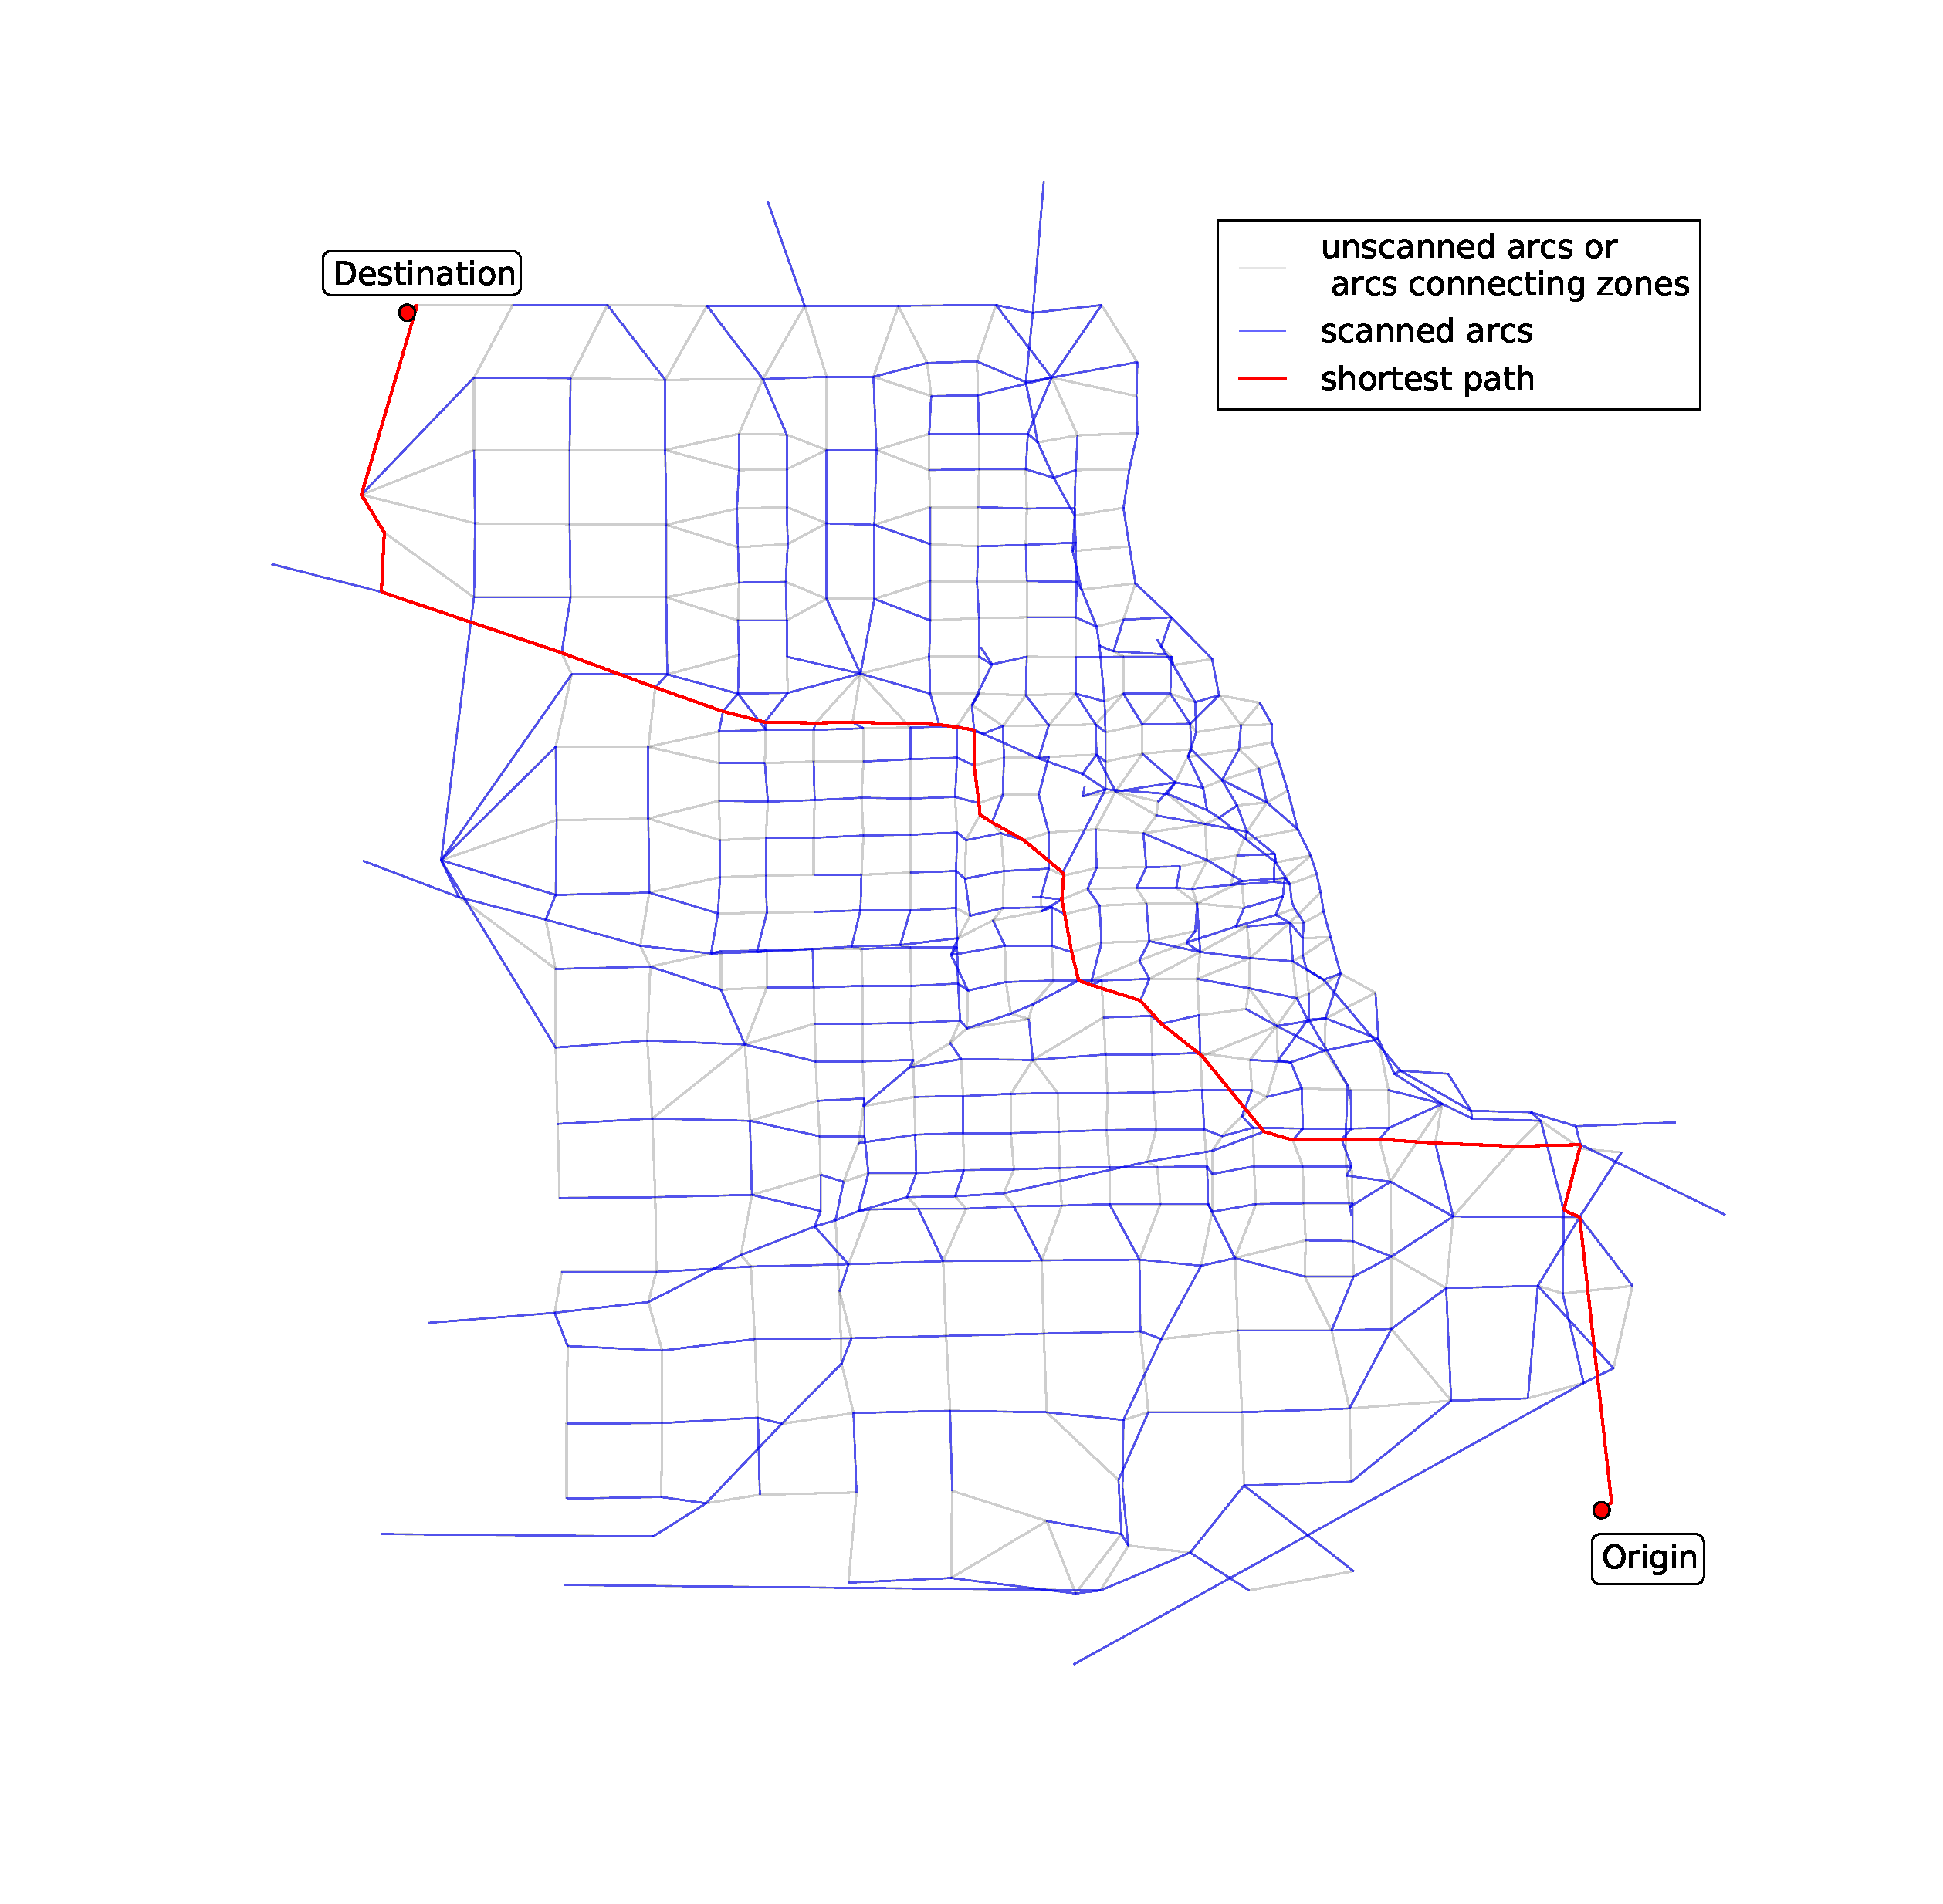
\includegraphics[width=\textwidth,trim=120px 120px 48px 120px,clip]{img/chicago_dijkstra}
        \caption{Dijkstra}
        \label{fig:chicago_dijkstra}
    \end{subfigure}%
    \begin{subfigure}{.5\textwidth}
        \centering
        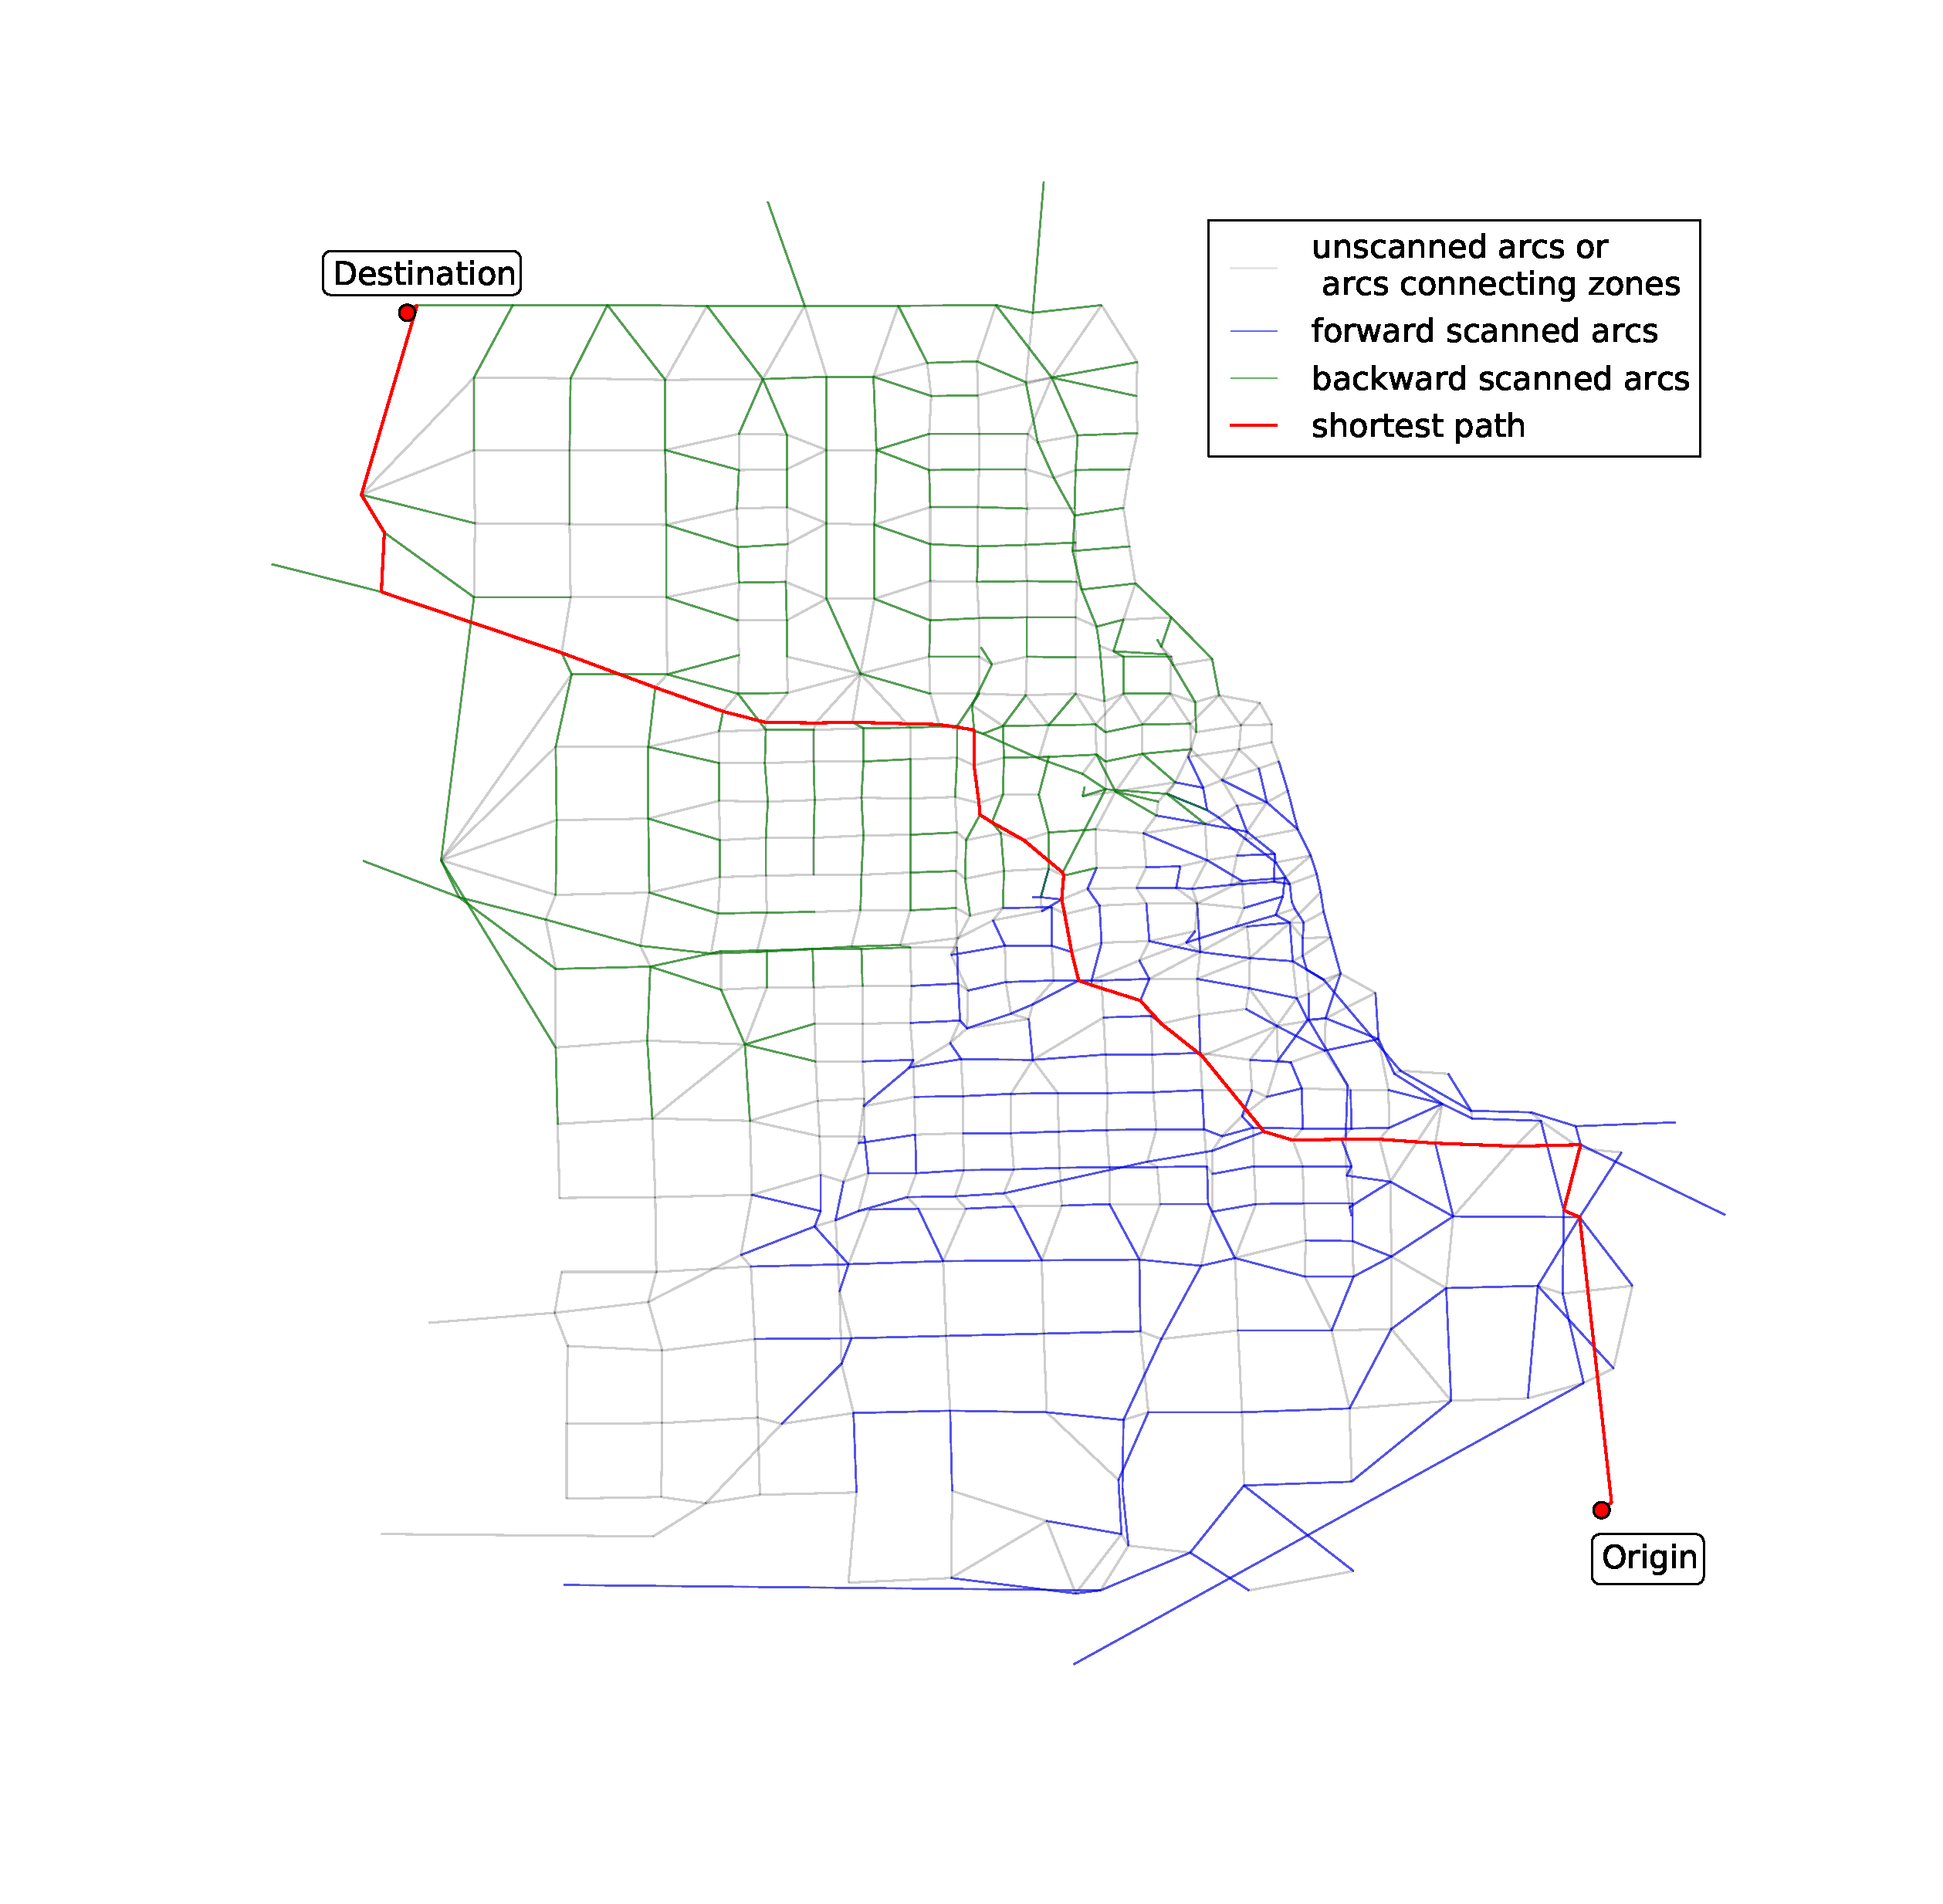
\includegraphics[width=\textwidth,trim=120px 120px 48px 120px,clip]{img/chicago_bidirect}
        \caption{Bidirectional Dijkstra}
        \label{fig:chicago_bidirect}
    \end{subfigure}
    \begin{subfigure}{.5\textwidth}
        \centering
        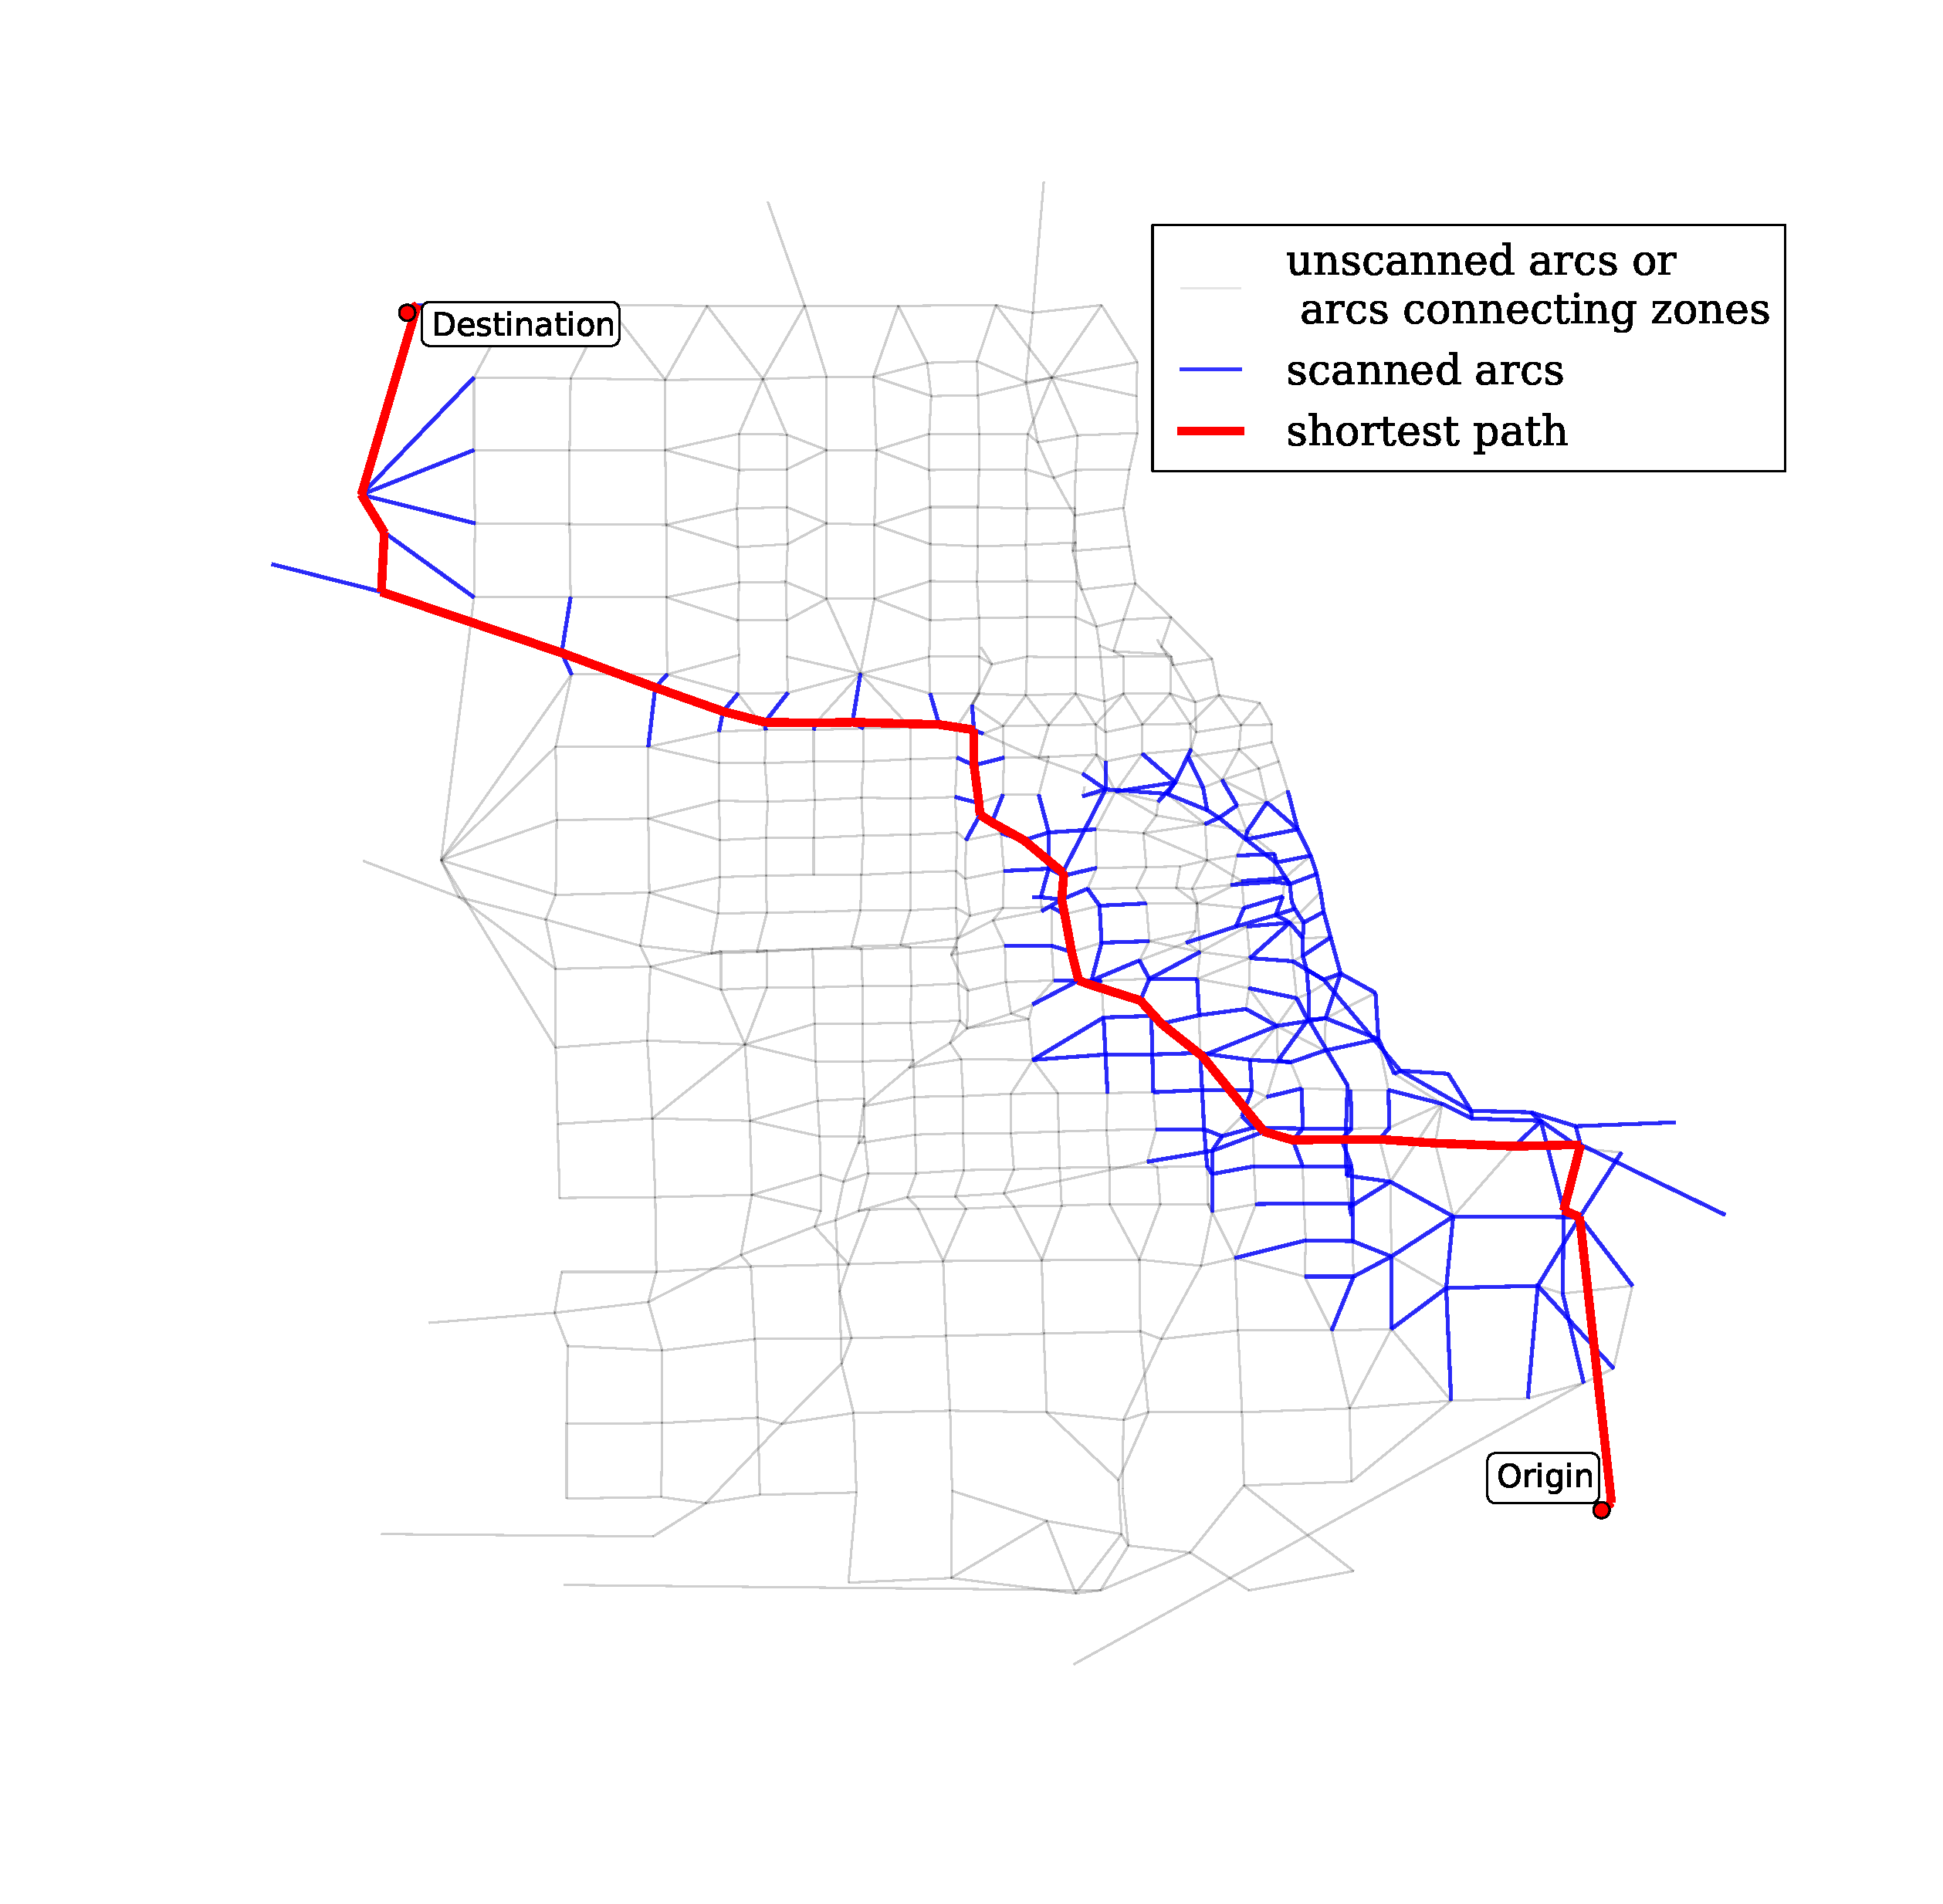
\includegraphics[width=\textwidth,trim=120px 120px 48px 0px,clip]{img/chicago_astar}
        \caption{A* Search}
        \label{fig:chicago_Astar_bidirect}
    \end{subfigure}%
    \begin{subfigure}{.5\textwidth}
        \centering
        \missingfigure[figwidth=\textwidth]{Bidirectional A*}
    %    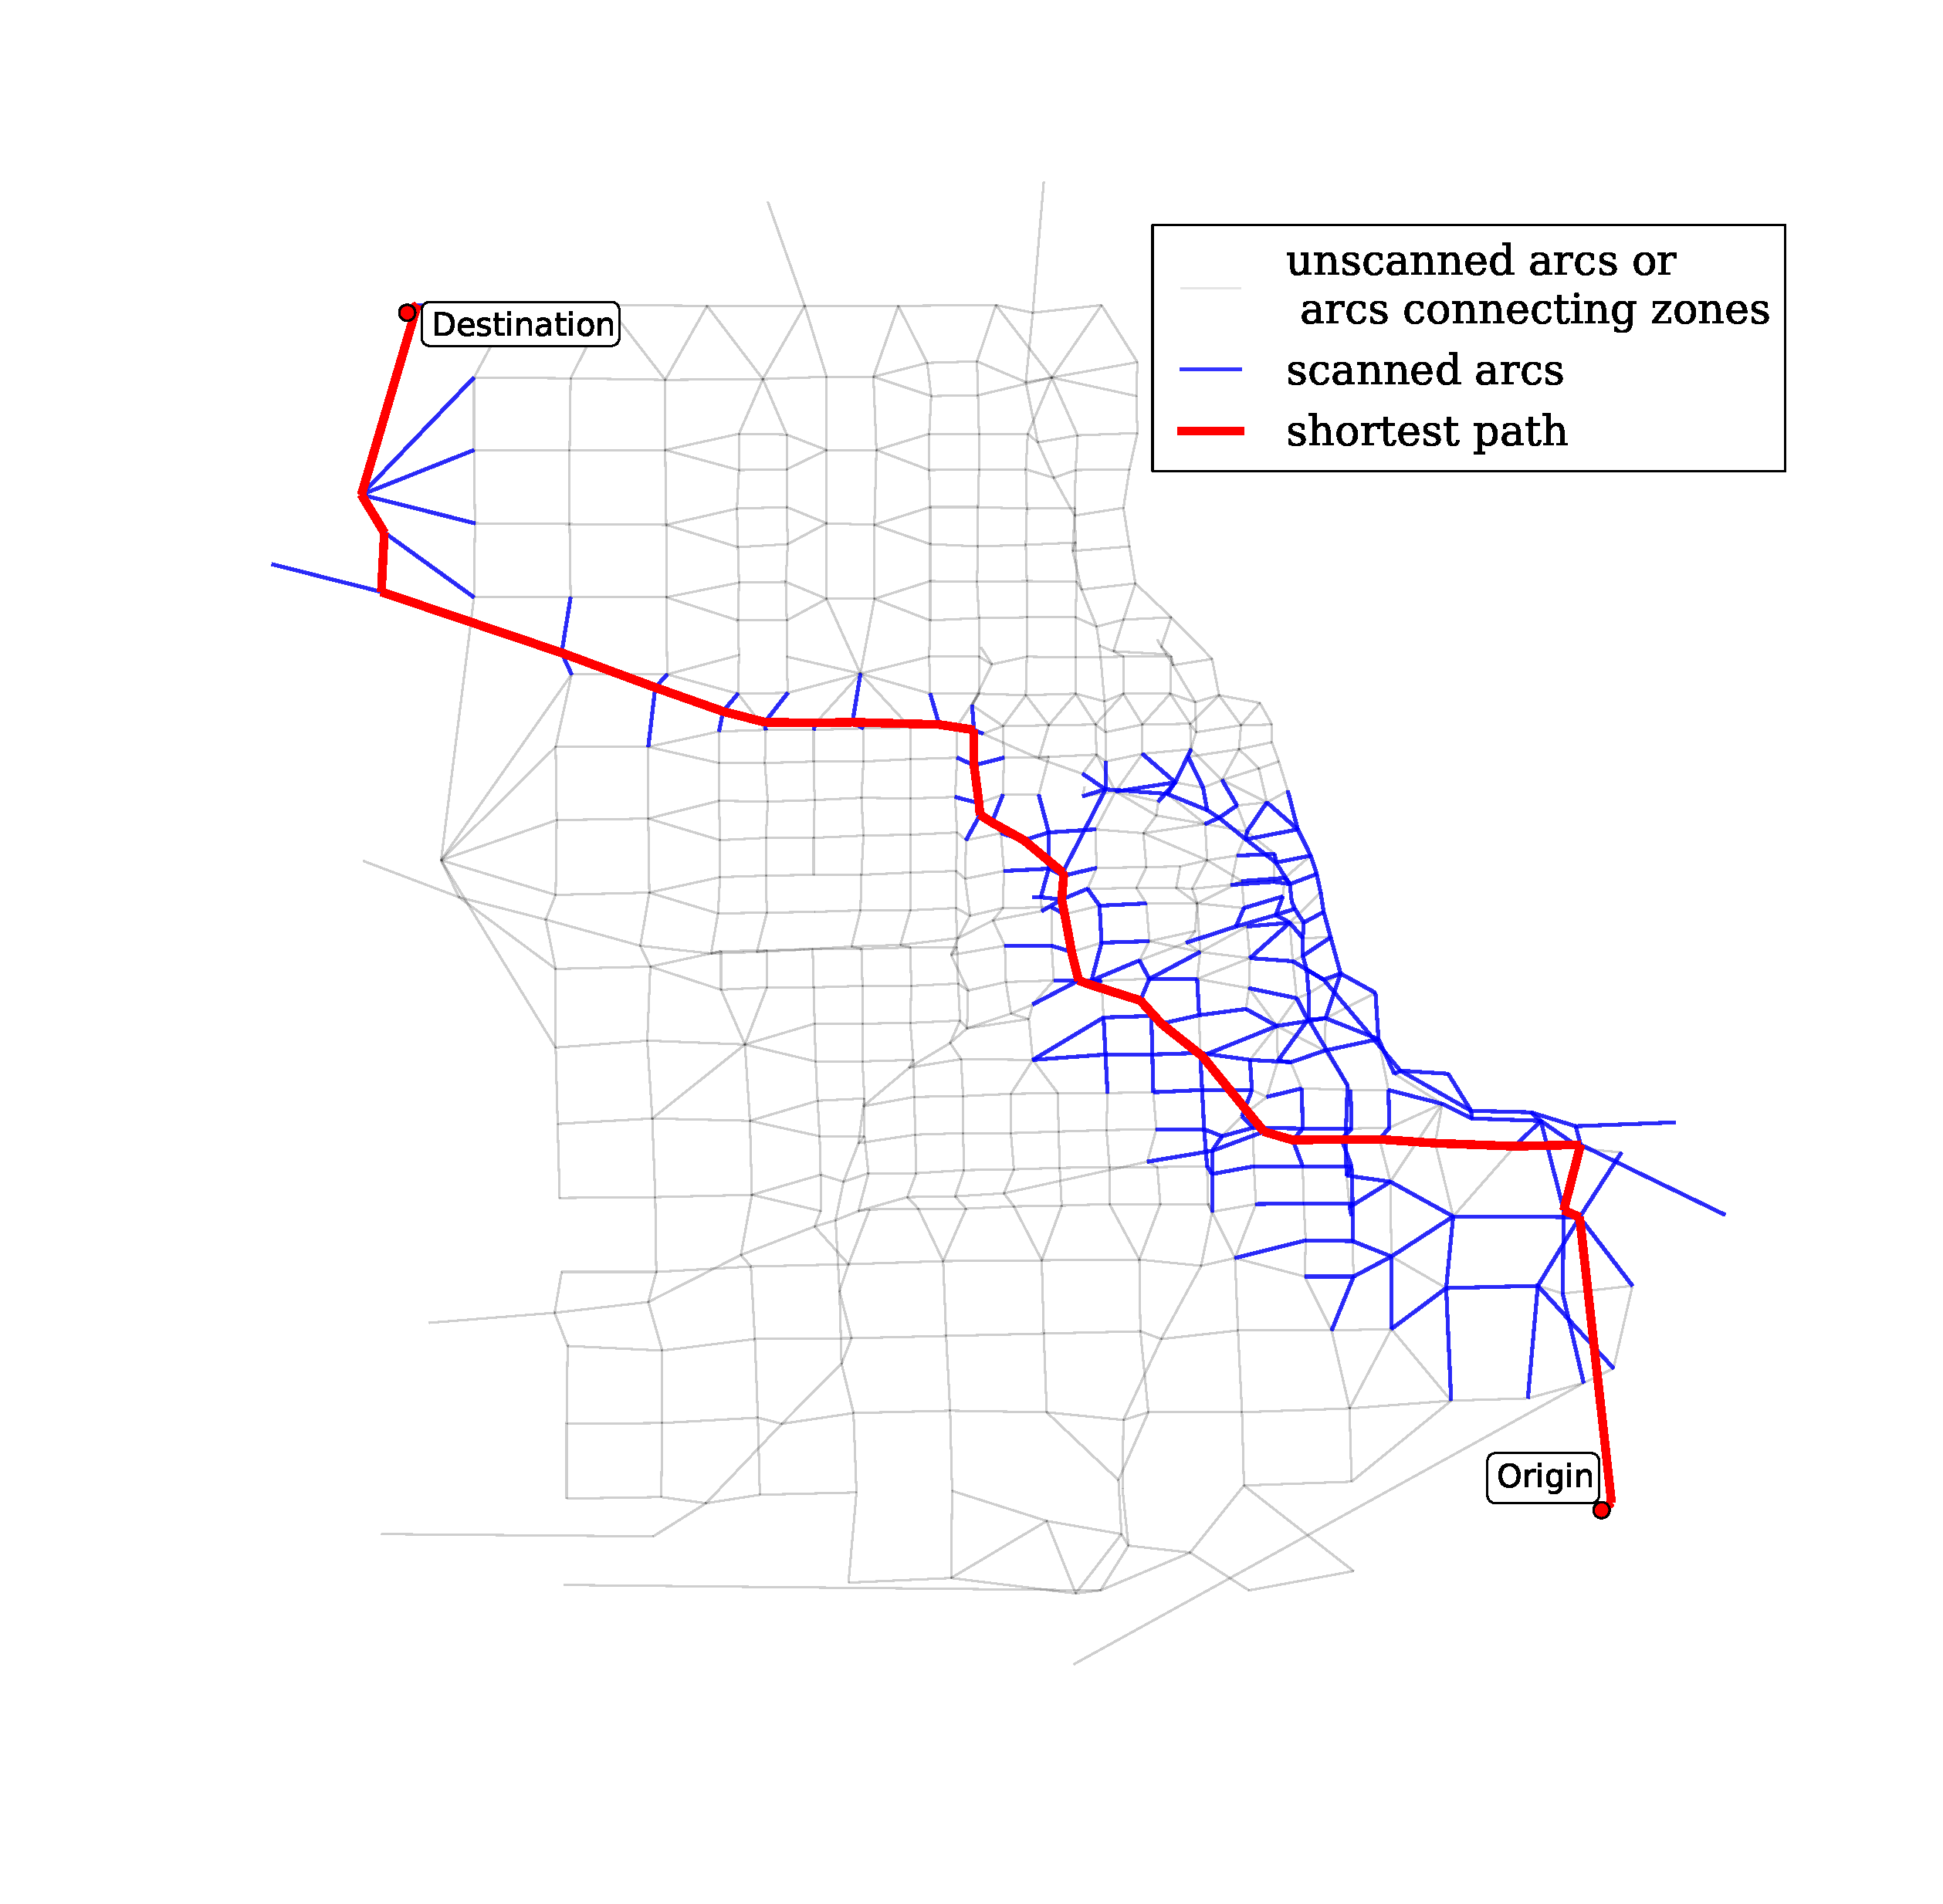
\includegraphics[width=\textwidth,trim=120px 120px 48px 0px,clip]{img/chicago_astar}
        \caption{Bidirectional A* Search}
        \label{fig:chicago_astar_bidirect}
    \end{subfigure}
    \vspace{1em}
    \caption{Shortest Path Tree for ChicagoSketch Network with Two Distant OD Pair}
    \label{fig:long_sptree}
\end{figure}
\todoin{draw 2 nodes that are close to each other}


\begin{comment}

All of these run times are slower than the STL version of the Heap.
Upon inspection,
it is found that the increase-key operation is used about between 5\% to 10\%
of the time,
\todo{not actual count yet}
which means the graphs are not dense enough for these Heap structures to outperform a
simple array based priority queue.
Comparing the Dijkstra and A* search algorithm's result,
we see an approximately 5 times improvement.
By looking at the shortest path tree generated
by the ChicagoSketch network,
there are only a few scanned nodes,
the path goes straight to the destination.
(TODO reference) says the closer the heuristic is to the actual distance,
the better/faster shortest path calculation,
by looking at the travel time function (Figure~\ref{fig:flowfunction}, we can see the slope
is really shallow near the start,
and by comparing the initial flow and final flow (TODO, data),
they are very close so the final flow is very close to the
initial flow,
which means the heuristic is a very good estimation,
which is our A* search is very fast.
\end{comment}


